% \note{These are tried to see if just features and some DP is enough to track beats and \gls{sama}. Mainly based on features Pre-2014 work: Onset detection, preliminary experiments on onset detection, HPSS, Akshara pulse tracking, and downbeat estimation (ICASSP 2014).}
The preliminary experiments around the task of meter analysis are exploratory experiments with existing features, rhythm descriptors, methods and algorithms to gain insights into the problem and test their relevance and utility in these tasks. The aim of including them in thesis is to gain useful insights and understand the limitations of those algorithms in meter analysis tasks for Indian art music. Only a selection of them are described here, primarily for Carnatic music, as a base for improved Bayesian models for meter analysis. We proposed a novel meter tracking algorithm in Carnatic music \cite{ajay:14:talaTrack} using pre-existing tools and rhythm descriptors, which is described in detail. The features and tools are explained as a part of the proposed meter tracking algorithm, emphasizing on their utility. 
%
\subsection[Meter tracking using dynamic programming]{Meter tracking using dynamic\\ programming}\label{sec:metertrack:dp}
The primary philosophy of meter tracking is to incorporate specific knowledge of the rhythmic structures we aim to estimate, which is also used in this approach. However, the approach aims to estimate the components of meter separately using a descriptor for each music concept. Using Carnatic music as an illustration, the algorithm estimates the \gls{akshara} period $\iai$, the \gls{akshara} pulse locations, and the \gls{sama}. For estimating these components, a set of rhythm descriptors are first computed from the audio that are indicative of the possible candidates for each musical concept. The periodicity and the relationships between these structures are then utilized to estimate the components. This framework can be generalized to estimating other rhythmic structures by suitably modifying the audio descriptor for the specific music culture and the rhythmic structure under consideration. 
\begin{figure}
  \centering
 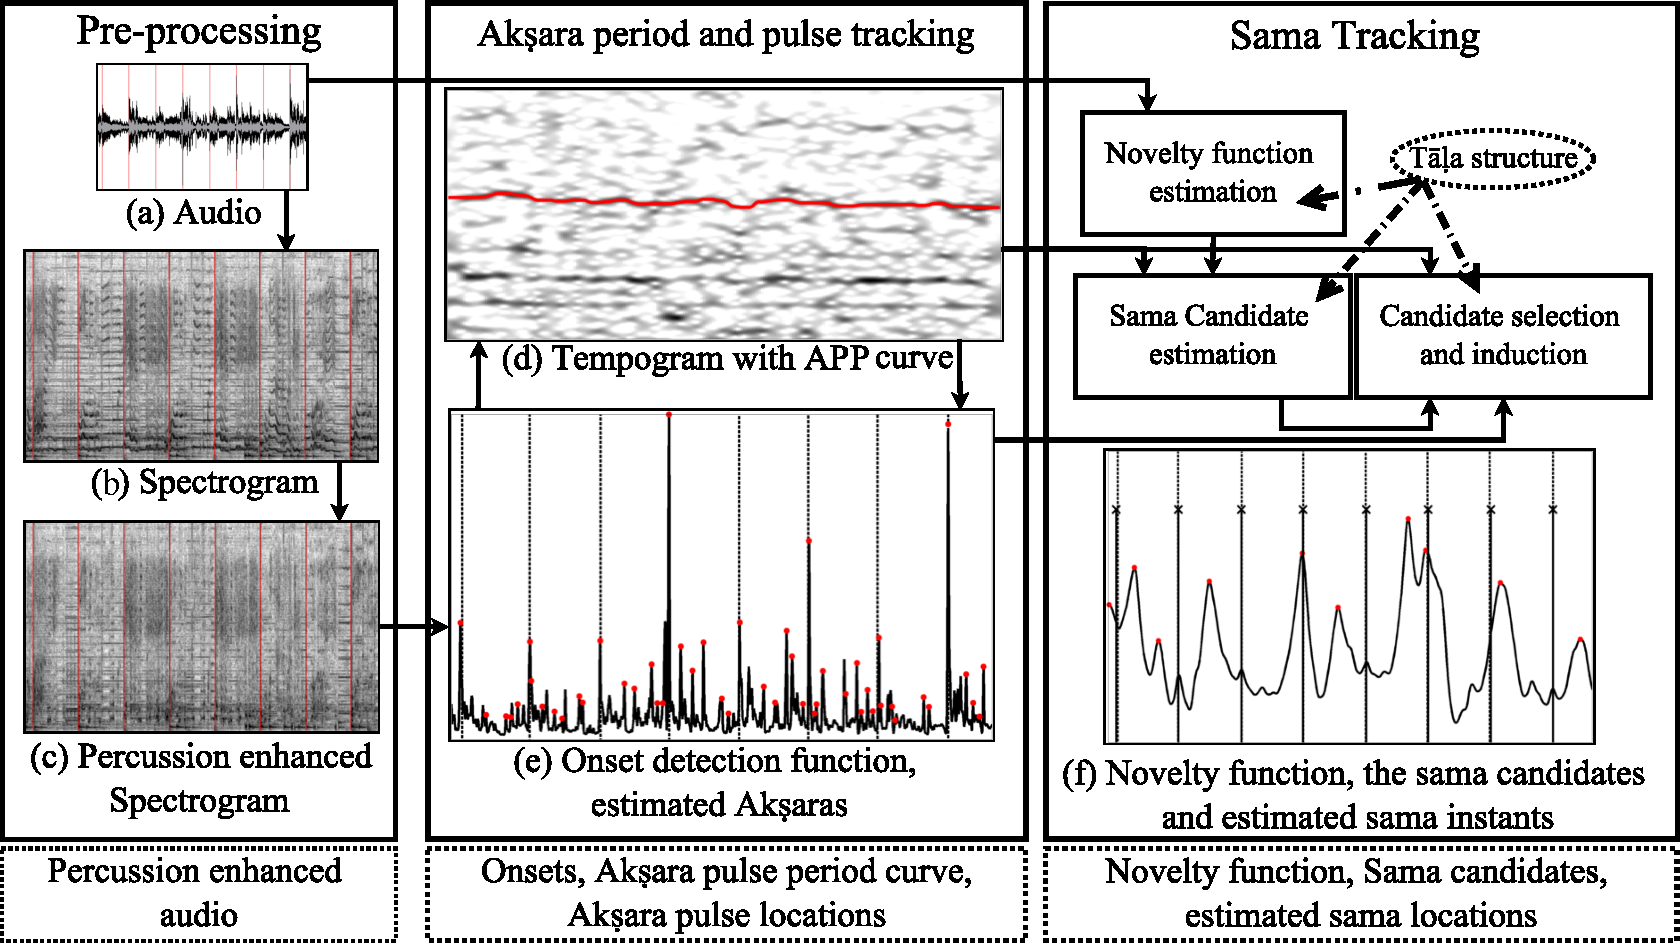
\includegraphics[width=\textwidth]{blockDiags/samaTrack-ICASSP-BlockDiag.pdf}
\caption[Block diagram of the \gls{tala} tracking algorithm proposed by \protect\citeA{ajay:14:talaTrack}]{Block diagram of the algorithm showing the signal flow and representative illustrations of different stages of the algorithm. The important outputs at each stage are also shown at the bottom. In each panel, the vertical lines that run through the panel indicate the \gls{sama} ground truth instants. The estimated \gls{sama}/\gls{akshara} candidates are shown with red dots and the estimated \gls{sama} are shown with $\times$.}\label{fig:BD:samaTrackICASSP}
\end{figure}

The algorithm for Carnatic music is explained in detail in this section. A hypothesis is that the \gls{akshara} pulses can be estimated from the onsets of mridangam, and hence a percussion onset based rhythm descriptor \cite{bello:05:onset} is useful for tracking the \gls{akshara} pulses. Tempogram\index{Tempogram}, a mid-level tempo representation for music signals proposed by \citeA{grosche:11:tempogram} is used to track the time-varying \gls{akshara} period. A novelty function\index{Novelty function} is computed using a self similarity matrix constructed using frame level onset and timbral features. These are then used to estimate possible \gls{akshara} and \gls{sama} candidates, followed by a candidate selection based on periodicity constraints, which leads to the final estimates. A block diagram of the approach is shown in \figref{fig:BD:samaTrackICASSP}. The features and the approach are explained further in detail. 
%
\subsubsection{Pre-processing: Percussion enhancement}
\begin{figure}
\captionsetup[subfigure]{labelformat=empty}
\centering
    \subfloat[]{\label{fig:preproc:hpssorg}
      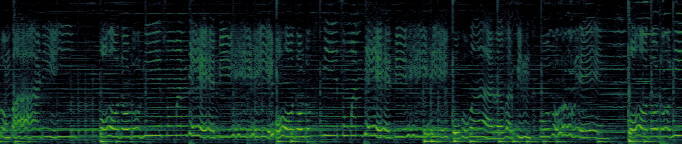
\includegraphics[width=0.95\textwidth]{meterTrack/HPSS-org.png}
    } \\ \vspace{-2em}
    \subfloat[]{\label{fig:preproc:hpssen}
      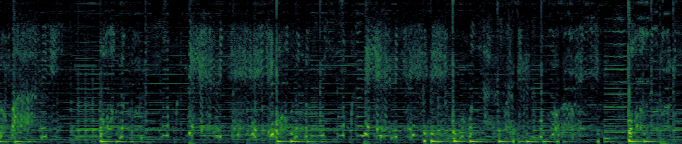
\includegraphics[width=0.95\textwidth]{meterTrack/HPSS-enhanced.png}
    } 
\caption[An illustration of percussion enhancement]{An illustration of percussion enhancement on a short audio excerpt of Carnatic music. The figure shows the spectrogram of the audio excerpt, before percussion enhancement (top panel) and after percussion enhancement by suppressing the lead melody (bottom panel). The lead melody is suppressed, while the \gls{tambura} (drone) is still present.}\label{fig:preproc:hpss}
\end{figure}
The \gls{akshara} pulse most often coincides with the onsets of mridangam strokes. To enhance the mridangam onsets, percussion enhancement is performed on the downmixed mono audio signal $\signal$ obtained from a music piece $\songVar$, as it has been shown to improve beat tracking performance in pieces with predominant vocals by \citeA{zapata:13:beatVS}. The predominant melody (\fzero)\index{Fundamental frequency} is estimated using the algorithm proposed by \citeA{salamon:12:melody} using which the harmonic component of the signal is extracted using a sinusoidal+residual model proposed by \citeA{serra:97:sms}. The percussion enhanced signal $\percsignal$, with the harmonic component suppressed, is used for further processing (\figref{fig:BD:samaTrackICASSP}(c)). An illustration of percussion enhancement for a short audio excerpt of Carnatic music is shown in \figref{fig:preproc:hpss}. 
%
\subsubsection{\Gls{akshara} period and pulse tracking}
\index{Tempo tracking}The spectrogram of $\percsignal$ is used to compute two frame level spectral flux\index{Spectral flux} based onset detection\index{Onset detection} functions \cite{bello:05:onset} computed every 11.6 ms. For each audio frame $k$ ($k \leq \nframes$), the first function ($\odfspfull$) uses the whole frequency range of the spectrogram and the other function computes the spectral flux only in the range of $0-120$ Hz ($\odfsplow$) and captures the low frequency onsets of the left (bass) drum head of the mridangam. 

The function $\odfspfull$ is used to compute a Fourier-based Tempogram $\tgMat$ proposed by \cite{grosche:11:tempogram}, computed every 0.25 second using a 8 second long window (\figref{fig:BD:samaTrackICASSP}(d)). If the time indexes at which the tempogram is computed is denoted with $i$, $(1\leq i \leq \nTGframes)$, the most predominant $\iai$ curve can be tracked by estimating the best path $\Gamma = \{\gamma_i: i = 1,2, \cdots, \nTGframes\}$ through the tempogram matrix $\tgMat$ that provides a balance between tempogram amplitude at time index $i$, $\tgMat_{\gamma_{_{i}},i}$, and the local continuity of $\iai$. An objective function, that is an extended version of the one used by \citeA{wu:11:beatDP}, is defined as shown in \eqnref{eqn:iai:icassp14}. 
%
\begin{equation}\label{eqn:iai:icassp14}
J_{1}\left(\Gamma,\theta_{1},\theta_{2}\right)=\underset{i=1}{\overset{\nTGframes}{\sum}}\tgMat_{\gamma_{_{i}},i}-\underset{i=1}{\overset{\nTGframes-1}{\sum}}\left(\theta_{1}\left|\gamma_{i}-\gamma_{i+1}\right|+\theta_{2}\;\Osym\left(\frac{\gamma_{i}}{\gamma_{i+1}}\right)\right) 
\end{equation}
The function $\Osym(\gamma_i/\gamma_{i+1})$ is an extra penalty term to penalize tempo doubling and halving between adjacent frames, and the parameters $\theta_1$ $(= 0.01)$ and $\theta_2$ $(= 10^6)$ provide different weights to the three terms. Based on observations from the \acrshort{CMDf} dataset, the search for the best path through the tempogram is restricted between the range of 120 to 600 APM (\glspl{akshara} per minute). 

The above objective function is solved using a \gls{DP} based approach to obtain a $\iai$ curve. Assuming the longest tracked $\iai$ curve to be at the correct metrical level, any possible tempo doubling/halving errors that are present are corrected to obtain the final curve $\Gamma^\optstar$ (\figref{fig:BD:samaTrackICASSP}(d), $\Gamma^\optstar$ is shown as a thick red line). Using the $\iai$ and the \gls{tala} information, we can obtain the time varying $\isi$ curve for the piece by multiplying the $\iai$ by the number of \glspl{akshara} in a cycle of the \gls{tala}. A further example of a tempogram and the estimated time varying $\iai$ curve for a piece of Carnatic music\footnote{Kamalamba, a \gls{kriti} in \gls{raga} Ānandabhairavi and \gls{mishra chapu} \gls{tala}, from the album Madrasil Margazhi 2005 by Aruna Sairam: \url{http://musicbrainz.org/recording/3baa722d-480e-4ae7-8559-a88dce41e1d4}} from \acrshort{CMDf} dataset is shown in \figref{fig:tempogram:app}. The figure shows the variations in tempo through a Carnatic music piece.
\begin{figure}
\centering
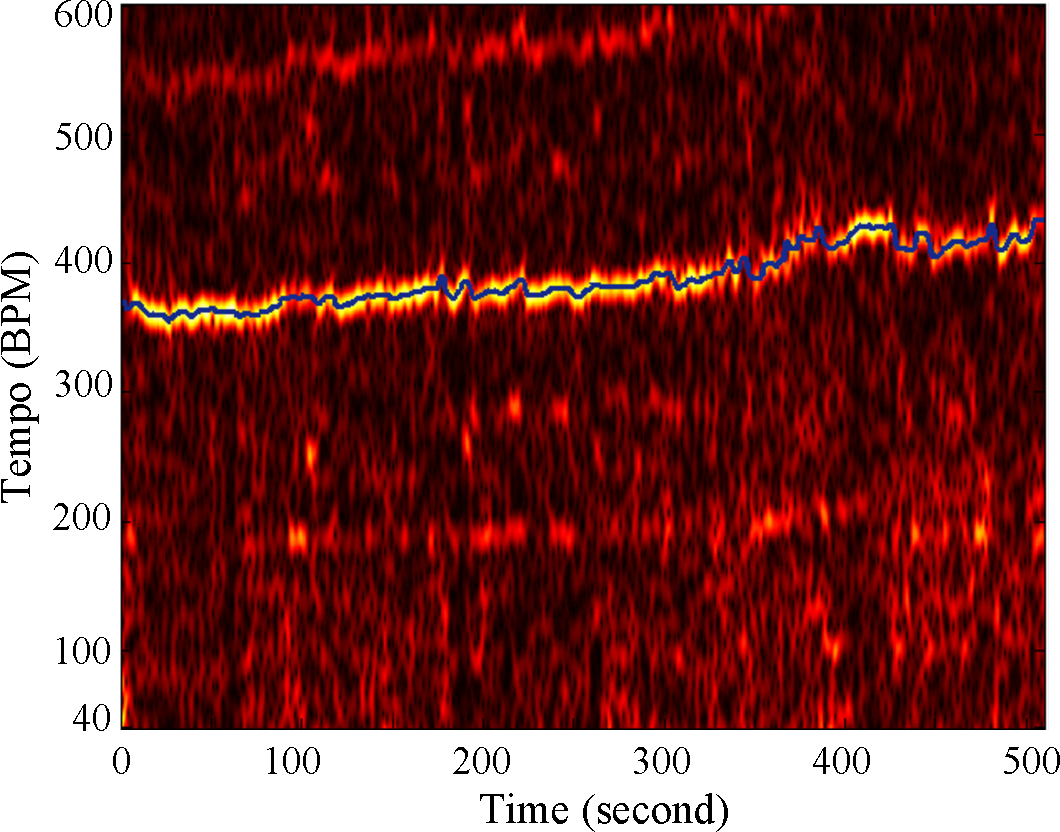
\includegraphics[scale=0.55]{meterTrack/tempogram-APP.pdf}
\caption[Estimated time varying tempo curve with tempogram]{Estimated time varying tempo curve (shown as a bold blue line) plotted on top of a tempogram, for a Carnatic music piece. In the piece, apart the local tempo variations, we can see that the tempo increases with time. The tempogram shows high values in tempo octave related bands, with the highest value (in yellow) at the estimated $\protect\iai$.}\label{fig:tempogram:app}
\end{figure}

The \gls{akshara} pulse locations predominantly lie on strong mridangam onsets. The \gls{akshara} pulse candidates are estimated as the peaks of the function $\odfspfull$. Using these $\kappa$ candidate peaks $\left\{o_i\right\}$, $i=1,2,3,\cdots,\kappa$, with locations $t_{i}$ and peak amplitude $\xi_{i}$, a cost function is setup as shown in \eqnref{eqn:AkCandEst:icassp14} to select the best candidates that provide a balance between the amplitude of these candidates and a periodicity provided by the estimated \gls{akshara} period. The best set of candidates $\aksSet = \left\{o^{\optstar}_i\right\} \subset \left\{o_i\right\}$ are estimated using a \gls{DP} approach (\figref{fig:BD:samaTrackICASSP}(e)).
\begin{equation}
\label{eqn:AkCandEst:icassp14}
J_{2}\left(\{o_{i}\},\delta\right)=\underset{i\subset \{1,2,\cdots, \kappa\}}{\sum}\left(\xi_{i}+\delta \, \Upsilon(t_{i},t_{i+1},\Gamma)\right)
\end{equation}
The function $\Upsilon(t_{i},t_{i+1},\Gamma)$ is a function that returns an exponentially decaying weight based on the time difference between $t_{i}$ and $t_{i+1}$ in relation to the local \gls{akshara} period, $\gamma_{t_k}$. The parameter $\delta(=3)$ provides a tradeoff between the two terms. 
\subsubsection{\Gls{sama} tracking}
%As described earlier, the samas are often associated with significant melodic, rhythmic and timbral changes. 
The use of \gls{MFCC} as features for timbral characteristics is explored. As a detection function for \gls{sama} ($\sdfsp$), a novelty function is computed through the diagonal processing of a self similarity matrix\index{Similarity matrix} \cite{foote:00:novelty} constructed using frame level z-score \gls{MFCC} features from audio (using audio processing library \textit{Essentia}~\cite{bogdanov:13:essentiaISMIR}) as shown in \figref{fig:BD:samaTrackICASSP}(f). Based on the $\overline{\isi}$ shown in \tabref{tab:datastat:cmdf}, a checkerboard kernel with size of 7, 3, 4, and 3 seconds is used for the \glspl{tala} \gls{adi}, \gls{rupaka}, \gls{mishra chapu} and \gls{khanda chapu} respectively so that the novelty function is computed over about an \gls{avartana}. 

The peaks of the novelty function $\sdfsp$ indicate a significant change of timbre at that time. Starting with the premise that timbral change is an important indicator of \gls{sama} location, the peaks of the novelty function are used to estimate \gls{sama} candidates. Two methods are explored to estimate the candidates. In Method-A, to uniformly choose \gls{sama} candidates throughout a piece, the piece is cut into segments of length 120, 40, 40 and 30 seconds for \gls{adi}, \gls{rupaka}, \gls{mishra chapu} and \gls{khanda chapu} respectively ($\sim$10 \glspl{avartana}), and the top five most prominent peaks in each segment of the piece are estimated as \gls{sama} candidates ($\{s^A_i\}$). 

Another approach, Method-B, is also proposed for candidate estimation that enforces a periodicity constraint while estimating \gls{sama} candidates. Starting from the peaks of $\sdfsp$ and estimated $\isi$ curve, for a specific peak, the \gls{tala} cycle is induced starting from it. The number of other peaks that would support such an induced \gls{tala} is assigned as the weight of the specific peak. The peaks are then rank ordered using this weight and the top ten ranked peaks are chosen as the \gls{sama} candidates ($\{s^B_i\}$). 

In addition, two random baseline methods RB-1 and RB-2 are created to compare the performance. In RB-1, a randomly chosen constant $\isi$ between 1-8 seconds is used, and a random starting time between 0-2 seconds to induce periodic \glspl{sama}. In RB-2, the estimated $\isi$ is used with 10 randomly chosen \gls{akshara} locations from $\{o_i\}$ as \gls{sama} candidates. RB-1 neither uses the $\isi$, nor the candidate estimation using $\sdfsp$, while RB-2 uses the estimated $\isi$ but not the candidate estimation using $\sdfsp$. 

Starting with the \gls{sama} candidates obtained either from Method-A or Method-B, for each candidate, the \gls{tala} cycles are induced based on local $\isi$ period obtained from the $\isi$ curve. For each seed, the next and previous three estimated cycle periods are searched for onset peaks in $\odfspfull$ that support a \gls{sama}. If a supporting onset is found, it is marked as a \gls{sama} and the algorithm proceeds further with the new estimated onset as the new anchor. The induction is stopped from a candidate when it does not lead to such a supporting onset. For each candidate, an estimated \gls{sama} sequence is thus obtained. Since all candidates are not necessarily \gls{sama} locations, though the estimated $\isi$ is right, the sequences can have different offsets. 

The final step of the algorithm is to shift, align and merge these sequences obtained from each candidate. Starting with the longest \gls{sama} sequence that has been estimated, other sequences are merged into this based on maximum correlation between the sequences. The merging of these sequences often leads to many \gls{sama} estimates concentrated around the true location of \gls{sama} due to small offsets. Since the left bass onsets on the mridangam are often strong at the \glspl{sama}, all groups of \gls{sama} estimates that are closer than 1/3\tsup{rd} of $\isi$ are merged into a single \gls{sama} estimate aligned with the closest left stroke onset obtained from $\odfsplow$. This forms the final set of \gls{sama} locations $\samaSet = \{s_{t_i}\}$ estimated from the candidates and the onset detection function, as shown in \figref{fig:BD:samaTrackICASSP}(f) with $\times$. 
\subsubsection{Results}
The annotated \acrshort{CMDf} dataset has annotations only for beats and \glspl{sama} of the piece. From the \gls{sama} locations, we can obtain the ground truth for $\isi$ curve, and hence the ground truth for $\iai$ curve. Since we do not have the ground truth for \gls{akshara} locations, we present the results only for tempo ($\iai$) and \gls{sama} tracking. 
\begin{table}
\centering
\begin{tabular}{@{}lcc@{}}\toprule
Measure & \gls{CML} & \gls{AML} \tabularnewline \midrule
$\overline{\iai}$ estimation & 81.2 & 98.9 \tabularnewline
$\iai$ tracking & 80.4 & 96.3 \tabularnewline \bottomrule
\end{tabular}
\caption[Results of \protect\gls{akshara} period tracking on \protect\acrshort{CMDf} dataset]{Accuracy (\%) of \protect\gls{akshara} period tracking on the \protect\acrshort{CMDf} dataset. The values are measured using a 5\% tolerance, at both correct metrical level (\gls{CML}) and allowed metrical levels (\gls{AML}).}\label{tab:APPtrack:icassp14}
\end{table}

The performance of \gls{akshara} period tracking is measured by comparing the ground truth \gls{akshara} period curve with the estimated curve with an error tolerance of 5\%. The results of median \gls{akshara} period estimation computed from the whole \gls{akshara} period curve of the piece is also reported. Further, since there can be tempo doubling and halving errors, the accuracies are reported at the annotated correct metrical level (\gls{CML}) and then using a weaker \gls{AML} measure that allows tempo halving and doubling (\gls{AML} - allowed metrical levels). 

The results are presented in \tabref{tab:APPtrack:icassp14}. We see that an acceptable level accuracy is achieved at \gls{CML} for both median \gls{akshara} period estimation and \gls{akshara} period tracking and further, there is not a significant difference between their performances, indicating that the algorithm can track changes in tempo effectively. Even when the \gls{akshara} period tracking fails at \gls{CML}, the algorithm tracks a metrically related \gls{akshara} period, as indicated by a high \gls{AML} accuracy. 
\begin{table}
\centering
%\rowcolors{2}{}{gray!25}
\begin{tabular}{@{}lccccc@{}}\toprule
\textbf{Variant} & \precision & \recall & \fmeas & \infoGain\ (bits) & Cand. Accu. (\%)\tabularnewline \midrule
Method-A & 0.290 & 0.190 & 0.216 & 1.17 & 20.46\tabularnewline 
Method-B & 0.246 & 0.202 & 0.215 & 1.25 & 27.85\tabularnewline \addlinespace[3pt]
RB-1 & 0.155 & 0.175 & 0.137 & 0.40 & - \tabularnewline 
RB-2 & 0.228 & 0.200 & 0.206 & 1.11 & 15.3 \tabularnewline \bottomrule
\end{tabular}
\caption[Results of \protect\gls{sama} tracking on \protect\acrshort{CMDf} dataset]{Accuracy of \gls{sama} tracking. The measures $\precision$: Precision, $\recall$: Recall, $\fmeas$: f-measure, $\infoGain$: information gain, are shown. The values are mean performance over the whole \acrshort{CMDf} dataset. The last column shows the fraction (as a percentage) of the estimated \gls{sama} candidates that are true samas.}\label{tab:ISItracking:icassp14} % expressed in \% except for information gain, which is in bits
\end{table}

For \gls{sama} tracking, the accuracy of estimation is reported with a margin of 7\% the annotated $\isi$ of the piece. Given the ground truth and the estimated \gls{sama} time sequence, we use the common evaluation measures used in beat tracking - precision, recall, f-measure and information gain \cite{mckinney:07:beatEval} to measure the performance. The results are shown in \tabref{tab:ISItracking:icassp14}, which also shows the accuracy of \gls{sama} candidate estimation. The results for RB-1 and RB-2 show mean performance over 100 and 10 experiments for each piece, respectively. 

We see that the performance of \gls{sama} candidate estimation and \gls{sama} tracking is poor in general, with \glspl{sama} correctly tracked only in about a fifth of cases. The precision is higher than recall in all cases, and information gain is lower than a perceptually acceptable threshold \cite{zapata:12:beat}. Both methods perform better than RB-1, but have comparable results with RB-2, with a slightly better f-measure performance (statistically significant in a Mann–Whitney U test at $p=0.05$). This shows that the estimated inter-\gls{sama} interval ($\isi$) is useful for \gls{sama} estimation, whereas candidate estimation using novelty function is only marginally useful. The poor performance can be mainly attributed to poor \gls{sama} candidate estimation with either of Method-A or Method-B. This is further substantiated by the fact that Method-B achieves an f-measure of 0.436 and an information gain of 1.70 bits when at least half the estimated candidates are true \glspl{sama}. This clearly shows that the performance of \gls{sama} tracking crucially depends on \gls{sama} candidate estimation. There are only four pieces (among all pieces with accurate $\isi$ estimation) in which all the estimated candidates are true \glspl{sama}, for which an f-measure of 0.894 and a information gain of 3.51 bits is achieved. This clearly indicates that the novelty function from which the \gls{sama} candidates were estimated is not a very good indicator of \gls{sama}, and better descriptors need to be explored. 
\subsubsection{Conclusions}

The presented approach to meter tracking with relevant rhythm descriptors for tempo, \gls{akshara}, and \gls{sama} and a hierarchical framework is promising, but has several limitations. The onset detection functions have information about surface rhythms and hence can be utilized for tempo tracking and \gls{akshara} pulse tracking, but the novelty function used presently is not a good indicator for sama. Further, it is observed that \gls{akshara} pulse period tracking performs to an acceptable accuracy for practical applications, while \gls{sama} tracking is challenging and performs poorly primarily due to poor \gls{sama} candidate estimation. 

Though tempo, \gls{akshara} and \gls{sama} are related, they were tracked separately. Even though information from tempo estimation was used in estimating the \gls{sama}, a joint estimation of the meter components is desired, since it can tightly couple these related components together. 

The approach uses the musical characteristics in isolation, without considering the interdependence between them. Further, many heuristic measures are used to track the components of the \gls{tala}. The learning from such heuristic approaches can be used to build a model that can more effectively model the underlying metrical structure, one that would consider the problem of meter inference and tracking more holistically. Such a model would also be adaptable to different metrical structures and handle variations in real world scenarios. The tracking algorithm based on dynamic programming is also ad hoc and loosely uses the tightly coupled information between the tempo, \glspl{akshara} and the \gls{sama}. 

Considering these insights and limitations, we explore Bayesian models for meter inference, which provide an effective probabilistic framework for the task, with several useful inference algorithms and well studied formulations that can be utilized to our benefit. The framework learns from training examples and hence the large number of heuristics used in these initial experiments become unnecessary. 
%
%\comment{We need better algorithms, and hence we use bayesian models for tracking!}
%
%1. Tracking each component in isolation is bad
%2. A model that truly is adaptable is needed, that reflects underlying metrical structure
%3. Onset kind of DF functions have some information and can be exploited
%4. Ad hoc approaches cannot be extended completely
%5. Learn from some of the pre-processing tools
%
%\note{Explain the experiments and results, emphasizing on how better models are needed.}